%******************************************************************************%
%**** pipeResolution - report *************************************************%
%**** 16th February 2017      *************************************************%
%**** daniel feldmann         *************************************************%
%**** pdflatex -> pdf         *************************************************%
%******************************************************************************%
%
%------------------------------------------------------------------------------%
\documentclass[a4paper, 11pt, twoside, DIV=12]{scrartcl}
%
%******************************************************************************%
%**** mtw2017 - proposal ******************************************************%
%**** 20th january 2017  ******************************************************%
%**** daniel feldmann    ******************************************************%
%**** pdflatex -> pdf    ******************************************************%
%******************************************************************************%
%
%--- font encoding ------------------------------------------------------------%
\usepackage[T1]{fontenc}                                                % output
\usepackage[utf8]{inputenc}                                              % input
% \usepackage{breakurl}
\usepackage[hyphens]{url}                  % avoid character clashes in email/web address
% \usepackage{}
%------------------------------------------------------------------------------%
%
%--- fonts --------------------------------------------------------------------%
\usepackage{palatino}                                                    % roman
\usepackage[scaled]{helvet}                                         % sans serif
\usepackage{courier}                                                % typewriter
\usepackage{eulervm}                                                      % math
\linespread{1.05}                                  % Palatino needs more leading
%------------------------------------------------------------------------------%
%
%--- modify title fonts -------------------------------------------------------%
\setkomafont{title}{\normalfont\bfseries}
\setkomafont{section}{\normalfont\bfseries\Large}
\setkomafont{subsection}{\normalfont\bfseries\large}
\setkomafont{descriptionlabel}{\normalfont\bfseries}
\setkomafont{caption}{\normalfont\footnotesize}
\setkomafont{captionlabel}{\normalfont\bfseries\footnotesize}
%------------------------------------------------------------------------------%
%
%--- language settings --------------------------------------------------------%
\usepackage[UKenglish]{babel}
%------------------------------------------------------------------------------%
%
%--- math, units and numbers --------------------------------------------------%
\usepackage{amsmath}
\usepackage{amssymb}
\usepackage{amstext}
\usepackage{dsfont}
\usepackage{mathtools}                                              % prescripts
\PassOptionsToPackage{decimalsymbol=.}{siunitx}
\PassOptionsToPackage{binary-units=true}{siunitx}
\usepackage{siunitx}
\usepackage{xfrac}
%------------------------------------------------------------------------------%
%
%--- colouring ----------------------------------------------------------------%
\usepackage[dvipsnames]{xcolor}                                    % make it gay
%------------------------------------------------------------------------------%
%
%--- useful command definitions -----------------------------------------------%
\usepackage{xspace}                       % get your subsequent spacing straight
\DeclareRobustCommand{\comment}[1]{\textit{\color{Gray}#1}\xspace}
\DeclareRobustCommand{\draft}[1]{\textit{\color{Red}#1}\xspace}
%------------------------------------------------------------------------------%
%
%--- cool pdf stuff -----------------------------------------------------------%
\PassOptionsToPackage{hyperindex}{hyperref}
\PassOptionsToPackage{breaklinks}{hyperref}                % useful for long url
\PassOptionsToPackage{hidelinks}{hyperref}          % remove ugly coloured boxes
\usepackage{hyperref}                      % hyperlinks for cross-refs and cites
\hypersetup{
 colorlinks,
 linkcolor={Maroon},
 citecolor={Maroon},
 urlcolor={Maroon}
}
%------------------------------------------------------------------------------%
%
%--- figures ------------------------------------------------------------------%
\RequirePackage{graphicx}
\RequirePackage{subfig}
% \usepackage{subfigure}           % obsolte, use subfig which provides subfloat
\RequirePackage{varwidth}            % to place several pics within one subfloat
% \usepackage{overpic}
% \addto\extrasUKenglish{\renewcommand{\figurename}{Fig.}}
%------------------------------------------------------------------------------%
%
%--- tables -------------------------------------------------------------------%
% \usepackage{tabularx}
\usepackage{booktabs}
\setlength{\extrarowheight}{0.2em}                     % increase table row height
% \usepackage{longtable}
% \usepackage{lscape}
% \usepackage{multirow}
% \usepackage{ragged2e}
% \newcolumntype{y}[1]{>{\RaggedLeft\arraybackslash\hsize=#1\hsize}X}
% \addto\extrasngerman{\renewcommand{\tablename}{Tab.}}
%------------------------------------------------------------------------------%
%
%--- bibliography -------------------------------------------------------------%
% \PassOptionsToPackage{authoryear, sort&compress}{natbib}
\PassOptionsToPackage{square, numbers}{natbib}
\usepackage{natbib}
% \usepackage{multibib}                      % more than one bib in one document
% \newcites{myPublications}{Publikationen}                   % define second bib
%------------------------------------------------------------------------------%
%
%--- index --------------------------------------------------------------------%
% \usepackage{makeidx}                                   % allows index generation
% \usepackage{multicol}                            % used for the two-column index
% \makeindex       % for subject index, use style svind.ist with makeindex program
%------------------------------------------------------------------------------%
%
%--- footnotes ----------------------------------------------------------------%
% \usepackage[bottom]{footmisc}                  % places footnotes at page bottom
%------------------------------------------------------------------------------%
%
%
%
\newcommand{\blackline}{\textcolor{black}{\protect\rule[0.5ex]{1.2em}{1pt}}}
\newcommand{\redline}{\textcolor{red}{\protect\rule[0.5ex]{1.2em}{1pt}}}
\newcommand{\blueline}{\textcolor{blue}{\protect\rule[0.5ex]{1.2em}{1pt}}}
\newcommand{\magentaline}{\textcolor{magenta}{\protect\rule[0.5ex]{1.2em}{1pt}}}
\newcommand{\orangeline}{\textcolor{orange}{\protect\rule[0.5ex]{1.2em}{1pt}}}
\newcommand{\cyanline}{\textcolor{cyan}{\protect\rule[0.5ex]{1.2em}{1pt}}}
%******************************************************************************%
%**** hff2016 - mathOperators *************************************************%
%**** 08th july 2016          *************************************************%
%**** daniel feldmann         *************************************************%
%**** pdflatex -> pdf         *************************************************%
%******************************************************************************%
%
%--- special characters -------------------------------------------------------%
\newcommand{\increment}{\,d\!}
\DeclareRobustCommand{\imag}{\ensuremath{\dot{\imath}}\xspace}  % imaginary unit
\DeclareRobustCommand{\orderof}{\ensuremath{\mathcal{O}}\xspace}     % magnitude
\DeclareRobustCommand{\real}{\ensuremath{\mathcal{R}}\xspace}        % real part
%------------------------------------------------------------------------------%
%
%--- non-dimensional numbers --------------------------------------------------%
\DeclareRobustCommand{\Courant}{\ensuremath{C\!o}\xspace}       % Courant number
\DeclareRobustCommand{\Mach}{\ensuremath{M\!a}\xspace}             % Mach number
\DeclareRobustCommand{\Reynolds}{\ensuremath{Re}\xspace}       % Reynolds number
\DeclareRobustCommand{\ReDelta}{\ensuremath{R\!e_{\delta}}\xspace}
\DeclareRobustCommand{\ReTau}{\ensuremath{R\!e_{\tau}}\xspace}
\DeclareRobustCommand{\ReTauStar}{\ensuremath{R\!e_{\tau}^{*}}\xspace}
\DeclareRobustCommand{\Strouhal}{\ensuremath{S\!t}\xspace}     % Strouhal number
\DeclareRobustCommand{\Womersley}{\ensuremath{W\!\!o}\xspace} % Womersley number
%------------------------------------------------------------------------------%
%
%--- special variables --------------------------------------------------------%
\DeclareRobustCommand{\ir}{\ensuremath{k_{\text{ir}}}\xspace}             % implicit radius
\DeclareRobustCommand{\tauw}{\ensuremath{\tau_{\text{w}}}\xspace}         % wall shear stress
\DeclareRobustCommand{\tauwStar}{\ensuremath{\tau_{\text{w}}^{*}}\xspace} % effective wall shear stress
\DeclareRobustCommand{\tauwsw}{\ensuremath{\tau_{\text{w,SW}}}\xspace}    % wall shear stress, Sexl-Womersley
\DeclareRobustCommand{\ubulk}{\ensuremath{u_{\text{b}}}\xspace}           % bulk velocity
\DeclareRobustCommand{\ubulksw}{\ensuremath{u_{\text{b,SW}}}\xspace}      % bulk velocity, Sexl-Womersley
\DeclareRobustCommand{\upeak}{\ensuremath{u_{\text{p}}}\xspace}           % peak bulk velocity
\DeclareRobustCommand{\upeaksw}{\ensuremath{u_{\text{p,SW}}}\xspace}      % peak bulk velocity, Sexl-Womersley
\DeclareRobustCommand{\utau}{\ensuremath{u_{\tau}}\xspace}                % friction velocity
\DeclareRobustCommand{\utauStar}{\ensuremath{u^{*}_{\tau}}\xspace}        % friction velocity
%------------------------------------------------------------------------------%
%
%--- indices ------------------------------------------------------------------%
\newcommand{\analytical}{\text{ana}}
\newcommand{\characteristic}{c\!h\!a}
\newcommand{\constant}{\text{const}}
\newcommand{\critical}{\text{krit}}
\newcommand{\initial}{i\!n\!i}
\newcommand{\numerical}{n\!u\!m}
\newcommand{\reference}{\text{ref}}
% \newcommand{\reference}{r\!e\!f}
\newcommand{\tidal}{t\!i\!d}
%------------------------------------------------------------------------------%
%
%--- finite volume sub/super scripts ------------------------------------------%
% \newcommand{\alphap}{\!\alpha^{\!+}}                              % alpha plus
% \newcommand{\alpham}{\!\alpha^{\!-}}                             % alpha minus
\newcommand{\betap}{\!\beta^{\!+}}                                   % beta plus
\newcommand{\betam}{\!\beta^{\!-}}                                  % beta minus
\newcommand{\betapm}{\!\beta^{\!\pm}}                          % beta plus minus
%------------------------------------------------------------------------------%
%
%--- functions ----------------------------------------------------------------%
\DeclareRobustCommand{\Bessel}{\ensuremath{\mathcal{J}_{0}}\xspace} % Bessel's function of first kind and order zero
% \DeclareRobustCommand{\Bessel}{\ensuremath{J_{0}}\!\!}         % Bessel's function of first kind and order zero
\renewcommand{\cos}{\operatorname{cos}}  % {c\!o\!s\!}
\renewcommand{\cosh}{c\!o\!s\!h}
% \renewcommand{\max}{m\!a\!x}
\DeclareRobustCommand{\Real}{\ensuremath{\mathcal{R}}\xspace}   % real part of a complex
\renewcommand{\sin}{sin\!}
%------------------------------------------------------------------------------%
%
%--- vector operators ---------------------------------------------------------%
\renewcommand{\vec}{\boldsymbol}
\newcommand{\divergence}{\operatorname{div}} %{d\!i\!v\!}
\newcommand{\gradient}{\operatorname{grad}} %{g\!r\!a\!d}
\newcommand{\laplacian}{\vec{\Delta}}
\usepackage{rotating}                                        % provides sideways
\renewcommand{\nabla}{\begin{sideways}\begin{sideways}$\laplacian$\end{sideways}\end{sideways}}
%------------------------------------------------------------------------------%
%
%--- relations ----------------------------------------------------------------%
\newcommand{\constraint}{\stackrel{!}{=}}
%------------------------------------------------------------------------------%
%
%--- statistical average delimiter --------------------------------------------%
\DeclareRobustCommand{\lla}{\left\langle}
\DeclareRobustCommand{\rra}{\right\rangle}
%------------------------------------------------------------------------------%
%
%------------------------------------------------------------------------------%
\newcommand{\ascii}{\texttt{ascii}\xspace}
\newcommand{\idl}{\texttt{idl/gdl}\xspace}
\newcommand{\flowsi}{\texttt{flowsi}\xspace}
\newcommand{\fortran}{\texttt{fortran90}\xspace}
\newcommand{\fftw}{\texttt{fftw3}\xspace}
\newcommand{\mpi}{\texttt{mpi}\xspace}
\newcommand{\netcdf}{\texttt{netCDF}\xspace}
\newcommand{\of}{OpenFOAM}
%------------------------------------------------------------------------------%
%
%------------------------------------------------------------------------------%
\newcommand{\ie}{i.\,e.\,}
\newcommand{\Ie}{I.\,e.\,}
\newcommand{\eg}{e.\,g.\,}
\newcommand{\Eg}{E.\,g.\,}
%------------------------------------------------------------------------------%
%
%
%

%
%--- title set-up -------------------------------------------------------------%
\subject{\vspace{-2.0ex}}
\titlehead{Technical report}
\title{Spatiotemporal resolution for\\ turbulent pipe flow simulations}
\subtitle{\vspace{-2.0ex}}
% \date{\vspace{-2.0ex}}
\author{Daniel Feldmann%
\thanks{University of Bremen,
Center of Applied Space Technology and Microgravity (ZARM),
Am Fallturm 2, 28359 Bremen, Germany,
Email: \url{daniel.feldmann@zarm.uni-bremen.de}}
and Daniel Mor\'on%
\thanks{University of Bremen,
Center of Applied Space Technology and Microgravity (ZARM),
Am Fallturm 2, 28359 Bremen, Germany,
Email: \url{daniel.moron@zarm.uni-bremen.de}}
}
% \date{\vspace{-3.0ex}}
% \date{\normalsize\today}
% \date{\includegraphics[height=15.00mm]{figures/logoZarm}}
% \date{\includegraphics[height=15.00mm]{figures/logoUniBremen}}
%------------------------------------------------------------------------------%
%
\begin{document}
%
\maketitle
%
\section{Range of scales in turbulent pipe flow}
A turbulent flow field is constituted of many irregular eddies and structures of
many different sizes which all move and deform with different speed. Figure
\ref{fig:plotPipePhiCompare} shows instantaneous snapshots of a velocity field
in a pipe to give an idea of the range of different length scales of these
eddies. Comparing the contour plots for different Reynolds number also
demonstrates how this spectrum of scales becomes even larger with increasing
\Reynolds.
\begin{figure}[htb]
\centering
\subfloat[Low Reynolds number ($\Reynolds=\num{5300}$, $\ReTau=\num{180}$)]{
\begin{varwidth}{\linewidth}
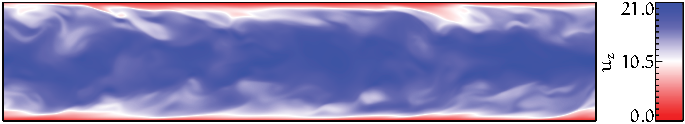
\includegraphics[width=1.00\textwidth]{figures/plotPipePhi-u2-ReTau0360.pdf}%\\
% 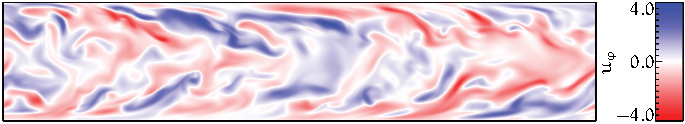
\includegraphics[width=1.00\textwidth]{figures/plotPipePhi-v2-ReTau0360.pdf}
\end{varwidth}
}\\
\subfloat[Moderate Reynolds number ($\Reynolds=\num{26000}$, $\ReTau=\num{720}$)]{
\begin{varwidth}{\linewidth}
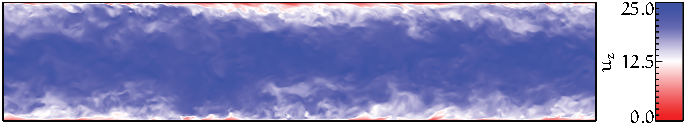
\includegraphics[width=1.00\textwidth]{figures/plotPipePhi-u2-ReTau1440.pdf}%\\
% 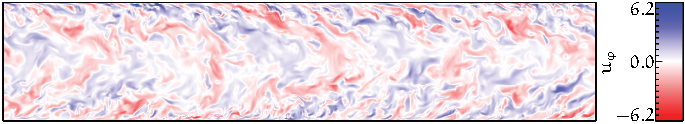
\includegraphics[width=1.00\textwidth]{figures/plotPipePhi-v2-ReTau1440.pdf}
\end{varwidth}
}
\caption{Comparison of turbulent pipe flow at two different Reynolds numbers to
illustrate the huge range of different length scales of eddies and structures in
the flow field. Shown are colour encoded contour plots of instantaneous
snapshots of the streamwise velocity component ($u_z$) in a longitudinal section
through the pipe taken from a DNS by Feldmann \cite{Feldmann2015c}. Here, $u_z$
is scaled in units of the shear velocity (\utau).}
\label{fig:plotPipePhiCompare}
\end{figure}
Figure \ref{fig:} shows time series of the streamwise velocity component
$u_z(\vec{x},t)$ at given locations $\vec{x}$ to illustrate the huge range of
time scales inherent to the turbulent flow field and its eddies and structures.
\par
In a direct numerical simulation (DNS) the number of spatial grid points is
determined by two constraints: First, the size of the computational domain must
be large enough to accommodate the largest scale of turbulent motion. Here, the
size can only be the length $L$ of the pipe domain in axial direction, since
there are natural constraints in azimuthal as well as in radial direction, which
are inherent to the pipe geometry. Second, the grid spacing must be sufficiently
fine to resolve the dissipative length scale, which is on the order of the
smallest scale of the turbulent motion. The cubed ratio of these two scales
provides a rough estimate for the total number of grid points ($N$) necessary
for sufficient spatial discretisation of the Navier-Stokes equations.
Additionally, the size of the discrete time step which is used to advance the
Navier-Stokes equations in time has to be small enough to resolve the fastest
fluctuations in the flow field. To set-up a well-resolved DNS of turbulent pipe
flow for a given \Reynolds, the size of the smallest time and length scales has
to be estimated a priori for this particular Reynolds number.
%
%
%
\section{Kolmogorov scales}
The characteristic scales of the smallest motions in a turbulent flow are the
Kolmogorov scales, see e.g. Pope \cite{Pope2000} page 185. These are the length
($\eta$), the time ($\tau_{\eta}$), and the velocity ($u_{\eta}$) scales formed
from dissipation rate $\epsilon$ and viscosity $\nu$ as follows:
\begin{align}
\eta &\equiv \left(\frac{\nu^{3}}{\epsilon}\right)^{\sfrac{1}{4}}
\label{eq:kolmogorovLengthScale}\\
\tau_{\eta} &\equiv \left(\frac{\nu}{\epsilon}\right)^{\sfrac{1}{2}}
\label{eq:kolmogorovTimeScale}\\
u_{\eta} &\equiv \left(\nu\epsilon\right)^{\sfrac{1}{4}}\text{.}
\label{eq:kolmogorovVelocityScale}
\end{align}
In preparation for a numerical simulation, the fluid property $\nu$ is in some
or another way know or given, e.g. by the control parameter \Reynolds. The
dissipation rate on the other hand, which is a property of the flow field and in
general a function of space and time ($\epsilon=f(\vec{x},t)$), is a priori
unknown and, therefore, has to be estimated to determine sufficient numerical
resolution in advance. Figure \ref{fig:} exemplarily shows dissipation rates
calculated in a DNS at $\ReTau=\num{720}$ \cite{}.
%
%
%
\section{Integral dissipation rate}
Since $\epsilon(\vec{x},t)$ is never know in advance, one can roughly
approximate (see e.g. Unger \cite{Unger1994}) that
\begin{align}
 \epsilon(\vec{x},t)\approx\lla\prescript{V}{}{\overline{\epsilon}}\rra_{t}\text{, where}
 \prescript{V}{}{\overline{\epsilon}} = \iiint\limits_{V}\epsilon(\vec{x},t)\increment V
\end{align}
represents a volume average over the entire computational pipe domain $V$.
The integral dissipation rate plotted figure \ref{fig} makes clear how rough
this estimate really is: Even in the temporal mean, dissipation in the pipe
changes with distance from the pipe wall, i.e. $\lla\epsilon\rra_{t}=f(r)$,
where $r$ is the radial direction in the cylindrical pipe flow coordinate
system. Near the pipe wall dissipation is larger than the integral value; in the
bulk region dissipation is somewhat smaller. Surely there will also be instantaneous deviations from the temporal
mean for all $r$ which might by larger. We will see later, that this estimate
is never the less very useful, if used carefully. Compare actual dissipation
profiles (averaged and instantaneous) from DNS data later on to discuss this\dots
\par
But the good thing is, that this integral value can be readily estimated from the pressure gradient

According to  the unknown dissipation rate
$\epsilon(\vec{x},t)$ can be approximated by the integral dissipation rate
 This quantity, in turn, can be readily
estimated from the usually known pressure gradient $\lla\sfrac{d p}{dz}\rra_{t}$
which drives the flow. This ansatz is based on the idea, that the total energy
input to the system --- basically the pressure gradient --- is eventually
dissipated into heat. Formally, this relation can be derived be integrating the
time-averaged budget equation for the total kinetic energy and neglecting direct
dissipation:
\begin{align}
\lla\frac{d p}{dz}\rra_{t}V\ubulk & =
\iiint\limits_{V}\rho\epsilon(\vec{x},t)\increment V =
\rho\prescript{V}{}{\overline{\epsilon}} V\\
\Rightarrow\qquad\prescript{V}{}{\overline{\epsilon}} & =
-\frac{1}{\rho}\lla\frac{d p}{dz}\rra_{t}\ubulk
\text{.}
\label{eq:volumeAveragedDissipation}
\end{align}

\par
In the Reynolds-averaged equations the pressure gradient and the wall-shear stress
\tauw balances out
\begin{align}
-\frac{1}{\rho}\lla\frac{d p}{dz}\rra_{t} =
\frac{4\tauw}{D\rho} =
\frac{4\utau^{2}}{D}\text{.}\label{eq:balanceOfForces}
\end{align}
From eq. (\ref{eq:volumeAveragedDissipation}) and eq. (\ref{eq:balanceOfForces})
it follows a simple relation
\begin{align}
\prescript{V}{}{\overline{\epsilon}} = \frac{4\utau^{2}\ubulk}{D}
\label{eq:dissipationVelocityRelation}
\end{align}
for the a priori unknown integral dissipation, which is basically a function of
\utau and \ubulk, since the pipe diameter $D$ is usually a known and constant
quantity.
%
%
%
\section{Shear to bulk velocity ratio}
Usually, in pipe flow simulations either \utau or \ubulk is a priori know while
the other one is an observed quantity, depending how the flow is driven through
the pipe in the numerical set-up. If the flow rate is kept constant during the
simulation, usually the bulk Reynolds number
\begin{align}
 \Reynolds=\frac{\lla\ubulk\rra_{t}D}{\nu}
 \label{eq:bulkReynoldsNumber}
\end{align}
based on the mean bulk flow velocity $\lla\ubulk\rra_{t}$ is the relevant
control parameter in the code. Thus, \ubulk is a known and constant quantity
while \utau is a result. If on the other hand, the driving force (i.e. the
pressure gradient) is kept constant, usually the friction Reynolds number
\begin{align}
 \ReTau=\frac{\lla\utau\rra_{t}R}{\nu}=\frac{\lla\utau\rra_{t}D}{2\nu}
 \label{eq:shearReynoldsNumber}
\end{align}
based on the mean shear velocity $\lla\utau\rra_{t}$ is the relevant control
parameter in the code. Thus, $\lla\utau\rra_{t}$ is a known quantity, while
\ubulk is a result.
\par
For further details and a
comprehensive discussion on the different flow driving mechanisms in numerical
simulations see e.g. Quadria et al. \cite{Quadrio2016} and Hasegawa et al.
\cite{Hasegawa2014}, who also introduced a third alternative in which the power
input to the system is kept constant and thus neither\dots
\par
A well-known and by now well-established empirical relation between \ubulk and
\utau given by

was first published by Blasius \cite{Blasius1913} in 1939 based on extensive
experiments in turbulent pipe flow.

Friction law according to Blasius \cite{Blasius1913}
\begin{align}
 \lambda_{\text{Blasius}} = \num{0.3164}\cdot\Reynolds^{\sfrac{-1}{4}}
\end{align}
which is valid for $\num{2300}\lesssim\Reynolds<\num{100000}$. Darcy-Weisbach
\begin{align}
 p_2 -p_1 = \Delta p_{12}& =\frac{\rho}{2}\frac{L\cdot\lambda}{D}\ubulk^2
 \quad\text{with}\Delta z=L\\
 \frac{\Delta p}{\Delta z} =\frac{\partial p}{\partial z} & =\frac{\rho}{2}\frac{\lambda}{D}\ubulk^2
\end{align}


%
%
%
\section{Integral length scale}
Using the integral dissipation rate given by eq.~(\ref{eq:dissipationVelocityRelation}),
from eq.~(\ref{eq:kolmogorovLengthScale}) an integral (i.e. volume averaged)
Kolmogorov length scale
\begin{align}
 \prescript{V}{}{\overline{\eta}} =
 \left(\frac{\nu^{3}}{\prescript{V}{}{\overline{\epsilon}}}\right)^{\sfrac{1}{4}} =
 \left(\frac{D\nu^{3}}{4\ubulk\utau^{2}}\right)^{\sfrac{1}{4}}
 \label{eq:meanKolmogorovLengthScale}
\end{align}
can be defined. For turbulent wall bounded flows it is common and convenient to
express length scales in viscous units (also called wall or inner units) defined
by
\begin{align}
 y^{+}\equiv y\frac{\utau}{\nu}
 \label{eq:viscousLengthScale}
\end{align}
and commonly denoted by ${}^{+}$. With eq.~(\ref{eq:viscousLengthScale}) and
eq.~(\ref{eq:meanKolmogorovLengthScale}) we arrive at
\begin{align}
 \prescript{V}{}{\overline{\eta}}^{+} =
 \prescript{V}{}{\overline{\eta}} \frac{\utau}{\nu} & =
 \frac{\utau}{\nu}\left(\frac{D\nu^{3}}{4\ubulk\utau^{2}}\right)^{\sfrac{1}{4}}\nonumber\\
 & = \left(\frac{D\nu^{3}\utau^{4}}{4\nu^{4}\ubulk\utau^{2}}\right)^{\sfrac{1}{4}}\nonumber\\
 & = \left(\frac{1}{4} \frac{\utau}{\ubulk} \frac{D\utau}{\nu} \right)^{\sfrac{1}{4}}\nonumber\\
 & = \left(\frac{1}{2} \frac{\utau}{\ubulk} \frac{R\utau}{\nu} \right)^{\sfrac{1}{4}}\quad\text{with eq.~(\ref{eq:shearReynoldsNumber})}\nonumber\\
 & = \left(\frac{1}{2} \frac{\utau}{\ubulk} \ReTau \right)^{\sfrac{1}{4}}
 \label{eq:etaPlus}
\end{align}
for the mean Kolmogorov length scale expressed in inner units. Multiplying
eq.~(\ref{eq:etaPlus}) by eq.~(\ref{eq:shearReynoldsNumber}) we get an
expression for the mean Kolmogorov length scale expressed in outer units (i.e.
expressed in pipe radii $R$) in the form of
\begin{align}
 \prescript{V}{}{\overline{\eta}}^{+}\frac{1}{\ReTau} & =
 \left(\frac{1}{2}\frac{\utau}{\ubulk}\ReTau\right)^{\sfrac{1}{4}}\frac{1}{\ReTau}\quad\text{with eq.~(\ref{eq:shearReynoldsNumber})}\nonumber\\
 \prescript{V}{}{\overline{\eta}}^{+}\frac{\nu}{\utau R} & =
 \left(\frac{1}{2}\frac{\utau}{\ubulk}\ReTau\right)^{\sfrac{1}{4}}\ReTau^{-1}\quad\text{with eq.~(\ref{eq:viscousLengthScale})}\nonumber\\
 \prescript{V}{}{\overline{\eta}}\frac{\utau}{\nu}\frac{\nu}{\utau R} & =
 \left(\frac{1}{2}\frac{\utau}{\ubulk}\right)^{\sfrac{1}{4}}\ReTau^{\sfrac{1}{4}}\ReTau^{-1}\nonumber\\
 \frac{\prescript{V}{}{\overline{\eta}}}{R} & =
 \left(\frac{1}{2}\frac{\utau}{\ubulk}\right)^{\sfrac{1}{4}}\ReTau^{\sfrac{-3}{4}}
 \text{.}
\end{align}

%
%--- Kolmogorov length scale --------------------------------------------------%
\begin{table}
\centering
\caption[]
{Estimated mean Kolmogorov length scale $\prescript{V}{}{\overline{\eta}}$ for
selected Reynolds numbers, where the ratio of \Reynolds
to \ReTau is based on Blasius' empirical law. Length scales are given in inner
and in outer units.}
\label{tab:kolmogorovLengthScale}
% \begin{tabularx}{\textwidth}{rrrr}
 \begin{tabular}{rrrr}
 \toprule
 \Reynolds &
\ReTau &
{$\prescript{V}{}{\overline{\eta}}^{+}$}&
{$\frac{\prescript{V}{}{\overline{\eta}}}{R}$}\\
\midrule
  \num{5300} &  \num{180.4} & \num{1.574} & \num{8.725E-03}\\
 \num{11700} &  \num{360.7} & \num{1.826} & \num{5.062E-03}\\
 \num{25800} &  \num{720.6} & \num{2.118} & \num{2.939E-03}\\
 \num{59600} & \num{1499.3} & \num{2.478} & \num{1.653E-03}\\
\num{130000} & \num{2966.5} & \num{2.868} & \num{9.669E-04}\\
\bottomrule
\end{tabular}
% \end{tabularx}
\end{table}
%------------------------------------------------------------------------------%
%






%
%--- back matter --------------------------------------------------------------%
\bibliographystyle{plainnat}
% \bibliographystyle{abbrv}
\bibliography{report.bib}
%------------------------------------------------------------------------------%
%
\end{document}
%------------------------------------------------------------------------------%
%
%
%
